\chapter{基于轨迹的低秩降维方法}

本章我们将介绍本文所采用的基于轨迹的低秩降维方法在中心化场景下的原理及算法。这一方法建立在对于神经网络训练过程的低维轨迹假设\cite{li2022low}上,其在低秩降维训练上的性能在一定程度上为这一假设提供支撑。本章将从这一假设出发,介绍该算法的原理及实现细节,并提供了验证性实验作为参考。

\section{低维轨迹假设}

在现在神经网络的训练过程中,数以百万乃至上亿的参数、梯度在每一轮迭代过程中完成计算、更新。而模型的这些大量参数之间,存在着较强的互相关联,也便存在着大量冗余的数据,引起了研究者们探究是否能用独立变量(independent variable)来表示神经网络的参数,即以一组互不相关的变量来存储并表征神经网络模型参数的更新。在\parencite{li2018measuring}的工作中,研究者将有着62006个参数的LeNet\cite{lecun2015lenet}降维至2900维的子空间,并在CIFAR-10\cite{krizhevsky2009learning}上达到了$90\%$的精度。在此之上,\parencite{gressmann2020improving}针对神经网络不同部分分别降维,且在每一轮中均进行随机的投影,使得降维后仅需数百个独立变量,但对最终精度产生较大影响。

以上对于降维神经网络至少数独立变量的研究均未考虑模型在训练过程中的动态轨迹(trajectory),故\parencite{li2022low}的作者在其工作中提出低维轨迹假设(The Low-dimensional Trajectory Hypothesis):
\begin{hyp}[低维轨迹假设]\label{hyp:low_dimensional}
    对于有着$n$个参数的神经网络,其模型参数在训练过程中的训练轨迹可被$d$维子空间所覆盖,其中$d \ll n$。
\end{hyp}

假设\ref{hyp:low_dimensional}认为,模型在训练过程中在迭代优化过程中的参数变化在高维空间中可以形成一条轨迹,且该轨迹可以被投影到相对较低的维度中,且投影前后轨迹差异较小,即在低维空间中训练得到的模型性能接近高维空间下训练得到的模型。如图(TODO)所示,。。。。。


且\parencite{li2022low}的作者在其工作中提出动态线性降维(Dynamic Linear Dimensionality Reduction,DLDR)方法对这一假设进行了验证。在该降维压缩方法下,常见的模型大小在$0.27$M到$28.5$M的范围内的神经网络均可在$40$个独立变量的子空间内完成训练,得到的精度与在高维空间中训练结果接近。


\section{动态线性降维方法}

针对神经网络降维问题研究始终围绕着寻找合适的降维策略使得降维得到子空间能够尽可能涵盖原高维空间中的信息,且使目标子空间的各个维度互不相干。在满足假设\ref{hyp:low_dimensional}的情况下,降维得到的子空间应尽可能覆盖模型训练轨迹,即轨迹在子空间上的投影与原高维空间中接近。从这一点出发,动态线性降维方法选择对训练过程进行采样,根据采样得到的离散的训练过程获得降维矩阵。这一过程包含如下几个操作:
\begin{enumerate} 
    \item 在神经网络常规训练过程中进行$t$轮采样,保存每次采样时的模型参数,记为$[\mathbf{w}_1, \mathbf{w}_2, \dots, \mathbf{w}_t]$。其中,$\mathbf{w}_i$为训练第过程中第$i$次采样的模型参数,展平所有参数矩阵为向量形式即$\mathbf{w}_i \in R^{n\times 1}$,$n$为模型参数个数。
    \item {
        对保存的采样结果进行归一化,即计算采样结果均值
        \begin{equation}
            \overline{\mathbf{w}} = \frac{1}{t}\sum_{i = 1}^t{\mathbf{w}_i},
        \end{equation}
        
        得到
        \begin{equation}
            W = [\mathbf{w}_1 - \overline{\mathbf{w}}, \mathbf{w}_2 - \overline{\mathbf{w}}, \dots, \mathbf{w}_t - \overline{\mathbf{w}}].
        \end{equation}
    }
    \item \label{enm:dldr:reduction}确定一个用基底向量$P = [\mathbf{e}_1, \mathbf{e}_2, \dots, \mathbf{e}_d]$表征的$d$维子空间,使其能够包含轨迹矩阵$W$。
\end{enumerate}

结合低维轨迹假设,上述步骤中的模型参数量$n$通常远大于$d$和$t$。

在操作\ref{enm:dldr:reduction}中,需要使降维目标子空间基底$P$与轨迹矩阵$W$尽可能接近,即最小化轨迹矩阵各列与目标子空间的距离和。在以L2范数($l_2$-norm)表征距离的情况下,可形式化表示为最大化$W$在目标空间投影的方差(variance):

\begin{equation}
    \max_{P} \text{tr}\left(P^TWW^TP\right), \text{ s.t. } P^TP=I.
\end{equation}

上述优化问题即为一个标准的主成分分析(Principal Component Analysis,PCA)问题,可以通过对$WW^T$进行谱分解(spectral decomposition)进行求解。求解得到的特征向量按照特征值排序,前$d$个特征向量作为目标空间的正交基底,也就是降维后用于训练需要的$d$个独立变量。

然而,$WW^T$ 是一个大小为$n\times n$的矩阵,在存储上具有较大的困难($n$为模型的总参数个数),且求解主成分问题的谱分解过程中的计算量在现有计算能力下难以完成。但结合线性代数的知识我们可以知道:

\begin{equation}
    \text{rank}(WW^T) \le \min \left\{\text{rank}(W), \text{rank}(W^T)\right\}\le \min\{n, t\}.
\end{equation}

由于$n\gg t$,$WW^T$是一个低秩矩阵。从矩阵$W$的奇异值分解(singular value decomposition,SVD)角度考虑,得到:

\begin{equation}
    W = U\Sigma V^T,
\end{equation}

其中,$U = [\mathbf{u}_1, \mathbf{u}_2, \dots, \mathbf{u}_n], \Sigma = \text{diag}(\sigma_1, \sigma_2, \dots, \sigma_{t}), V = [\mathbf{v}_1, \mathbf{v}_2, \dots, \mathbf{v}_t]$。奇异值分解结果中的$U$的前$d$列即为我们所需要的独立向量。考虑到$W$和$W^T$具有相同的奇异值分解结果,我们可以通过对$W^TW$进行谱分解,得到$\mathbf{v}_i, i = 1\dots d$。由于$W^TW$是一个大小为$t\times t$的矩阵,计算复杂度大大降低。然后,通过下式计算出$\mathbf{u}_i, i = 1\dots d$。


\begin{equation}
    W\mathbf{v}_i = \sigma_i mathbf{u}_i, i= 1\dots d.
\end{equation}

将上述方法以伪代码形式表述于算法\ref{algo:dldr}中。

\begin{algorithm}[htb]
    \caption{动态线性降维方法}
    \label{algo:dldr}
    \small
    \SetAlgoLined
    \KwIn{采样数量$t$,目标子空间维度$d$}
    \KwOut{正交基底$[\mathbf{u}_1, \mathbf{u}_2, \dots, \mathbf{u}_d]$}
    在训练过程中采样模型轨迹$\{\mathbf{w}_1, \mathbf{w}_2, \dots, \mathbf{w}_t\}$\;

    $\overline{\mathbf{w}} = \frac{1}{t}\sum_{i = 1}^t{\mathbf{w}_i}$\;

    $ W = [\mathbf{w}_1 - \overline{\mathbf{w}}, \mathbf{w}_2 - \overline{\mathbf{w}}, \dots, \mathbf{w}_t - \overline{\mathbf{w}}]$\;

    在$W^TW$上进行谱分解,得到前$d$大的特征值$[\sigma_1^2, \sigma_2^2, \dots, \sigma_d^2]$,以及对应的特征向量$\mathbf{v}_1, \mathbf{v}_2, \dots, \mathbf{v}_d$\;

    $\mathbf{u}_i = \frac{1}{\sigma_i}W\mathbf{v}_i, i = 1 \dots, d$\;
    
    得到$[\mathbf{u}_1, \mathbf{u}_2, \dots, \mathbf{u}_d]$这一正交基底\;

  \end{algorithm}

在算法\ref{algo:dldr}中,总共需要进行对大小为$t\times t$的矩阵的一次谱分解和一次矩阵乘法,计算复杂度为$\mathcal{O}\left(t^3 + t^2n\right)$。其中矩阵乘法操作可以被图形处理器(GPU)显著加速,总时间消耗相比神经网络训练可以忽略。

\section{基于轨迹降维的训练算法}

本节中我们给出基于上述降维算法,在中心化单机器上训练神经网络训练过程,以验证动态线性降维方法获得的目标子空间是否能够支持神经网络的训练,即验证低维轨迹假设\ref{hyp:low_dimensional}的正确性。本文采用的算法分为三个阶段:采样阶段、降维阶段、训练阶段。

\subsection{采样阶段}

在这一阶段,在采样数据集上按随机梯度下降(stochastic gradient descent)进行常规模型训练,并按照固定间隔保存模型参数。总采样轮数$t$略大于目标子空间维度$d$。考虑到常规模型训练达到稳定后参数变化较小,故采样阶段应尽量覆盖模型快速收敛的阶段,不必采样至模型完全收敛,使得采样得到的模型轨迹信息更合理。


\begin{algorithm}[htb]
    \caption{轨迹采样算法}
    \label{algo:sgd_with_sampling}
    \small
    \SetAlgoLined
    \KwIn{采样数据集$D$,采样总数$t$,学习率$\eta$,批量大小$B$,单次采样批量数$M$,损失函数$L$}
    \KwOut{模型轨迹采样结果$\mathbf{w}_1, \mathbf{w}_2, \dots, \mathbf{w}_t$}
    随机初始化神经网络模型参数$\theta$\;
    \For{$i \leftarrow 1$\KwTo $t$} {
        \For {$j \leftarrow 1$\KwTo $M$} {
            从采样数据集$D$中随机抽取$B$个样本$x$\;
            $g \leftarrow \nabla_{\theta} L(\theta, x)$\;
            $\theta \leftarrow \theta - \eta g$\;
        }
        将神经网络模型参数$\theta$展平成一行,保存为$\mathbf{w}_i$\;
    }
    得到训练轨迹采样结果$\mathbf{w}_1, \mathbf{w}_2, \dots, \mathbf{w}_t$\;

  \end{algorithm}

\subsection{降维阶段}

在这一阶段,按照算法\ref{algo:dldr}的步骤从上一阶段的采样结果中执行降维,得到目标子空间的基底,也即降维矩阵$P$。


\subsection{训练阶段}

在这一阶段,我们在降维后的子空间中从头训练(from scratch)原有的模型。在每一轮迭代过程中,在使用随机梯度下降法计算得到当前批量(mini-batch)的梯度后,使用降维投影矩阵$P$将梯度投影至$d$维的目标子空间,得到长度为$d$的子空间梯度向量,作为我们降维压缩的结果。在更新模型参数时,考虑到学习率(learning-rate)映射到目标子空间需要额外的计算,且由于降维矩阵的线性性,在高维空间执行模型更新和在低维目标子空间进行梯度更新的效果是一致的,因此我们选择在高维空间进行模型更新。

将这一过程以伪代码的形式表述为算法\ref{algo:psgd}


\begin{algorithm}[htb]
    \caption{低秩降维训练算法}
    \label{algo:psgd}
    \small
    \SetAlgoLined
    \KwIn{降维压缩矩阵$P$,学习率$\eta$,批量大小$B$,单轮学习批量数$M$,总轮数$epoch$}
    \KwOut{完成训练的神经网络参数$\theta$}
    在上一阶段获得降维矩阵$P = [\mathbf{e}_1, \mathbf{e}_2, \dots, \mathbf{e}_d]$\;
    随机初始化神经网络模型参数$\theta_0$\;
    \For{$i \leftarrow 1$\KwTo $epoch$} {
        \For {$j \leftarrow 1$\KwTo $M$} {
            从采样数据集$D$中随机抽取$B$个样本$x$\;
            $g \leftarrow \nabla_{\theta_{i - 1}} L(\theta_{i - 1}, x)$\;
            将梯度投影到目标子空间:$\bar{g} \leftarrow P^Tg $\;
            将低维空间中的梯度信息重新映射回高维:$\widetilde{g} \leftarrow P\bar{g}$\;
            在高维空间进行更新:$\theta_{i} \leftarrow \theta_{i - 1} - \eta \bar{g}$\;
        }
    }
    得到训练完成的模型参数$\theta_t$\;
  \end{algorithm}


\section{中心化场景下实验部分}

为了验证低维轨迹假设,即验证算法\ref{algo:dldr}得到的降维目标子空间是否能用于神经网络的训练,我们将给出我们在中心化场景下完成的验证性实验。


\subsection{数据集}

我们采用了大规模的公开真实图像识别数据集CIFAR-10\cite{krizhevsky2009learning}作为我们的主要实验平台。

CIFAR-10数据集中一共有50000张训练图像和10000张测试图像,均为RGB三通道(channel)彩色图像,每张图像均有对应的标签。数据集中总共有十个类别,每个类别均有6000个图像:飞机(airplane)、机动车(automobile)、鸟(bird)、猫(cat)、鹿(deer)、狗(dog)、蛙(frog)、马(horse)、船舶(ship)和货车(truck)。 其中每个图像的尺寸均为$32 \times 32$,单位像素(pixel)。作为具有良好标注、划分均等的数据集,CIFAR-10常作为各类神经网络训练的评价指标,也在前述的各类降维相关研究\cite{li2018measuring}被使用,因此作为本小节实验的数据集较为合理。

在本小节的实验中,为了便于对比降维前后的神经网络性能差异,我们使用CIFAR-10同时作为轨迹采样数据集和低秩训练数据集。

\subsection{模型}

低维轨迹假设本身对于神经网络的模型架构没有特定的要求,理论上算法\ref{algo:dldr}适用于现有各类模型结构,仅不同架构中参数信息的交互程度在一定程度上影响降维的压缩率。在本节的验证实验中,我们选择了较为常用的Resnet-20\cite{he2016deep}作为实验的模型架构。

Resnet-20结构下的神经网络共有约$0.27$M个参数。


\subsection{实验设定}

在采样阶段,我们使用在轨迹采样数据集CIFAR-10上使用算法\ref{algo:sgd_with_sampling}训练Resnet-20。这一训练过程中使用的具体参数有:学习率(learning rate)为$0.1$,动量(momentum)参数为$0.9$,批量大小(batch size)为$128$。采样过程中,我们在训练每个轮次(遍历一轮轨迹采样数据集)后进行一次采样,总共进行$40$轮采样。同时,为了便于得到与常规SGD方法对照的结果,我们在采样$40$轮结束后仍进行训练达到$80$轮,在$40$轮到$80$轮的过程中不进行模型轨迹的采样与保存。

在降维阶段,我们使用算法\ref{algo:dldr}对上一阶段$40$轮采样结果进行降维以提取目标子空间,降维目标维度为$20$,得到降维矩阵$P$。

在训练阶段,我们在降维阶段得到的目标子空间中,在低秩训练数据集中按照算法\ref{algo:psgd}的方式进行训练。在这一阶段的训练中,低秩空间的模型参数为随机初始化得到,即从头训练(from scratch),避免采样阶段学习得到模型参数影响低秩训练阶段的结果。为了对比的公平性,在此处我们使用的训练参数和采样阶段使用的超参数相同。

\subsection{实验结果}

在采样阶段中,我们用于对照的常规随机梯度下降算法在第$80$轮内达到的最高测试精度为$88.63\%$。在采样结束时($40$轮),常规随机梯度下降算法达到的精度为$84.96\%$。

在降维阶段中,我们降维得到了投影目标子空间,我们将投影后的各个分量(component)中方差占比前$10$的具体数值展示在图\ref{fig:dldr:pca_ratio}中。可以观察到,前$5$个分量占据了降维后目标空间中超过$85\%$的总方差,这在一定程度上表明在低秩目标子空间中足够涵盖模型的训练轨迹。
\begin{figure}[!htp]
    \centering
    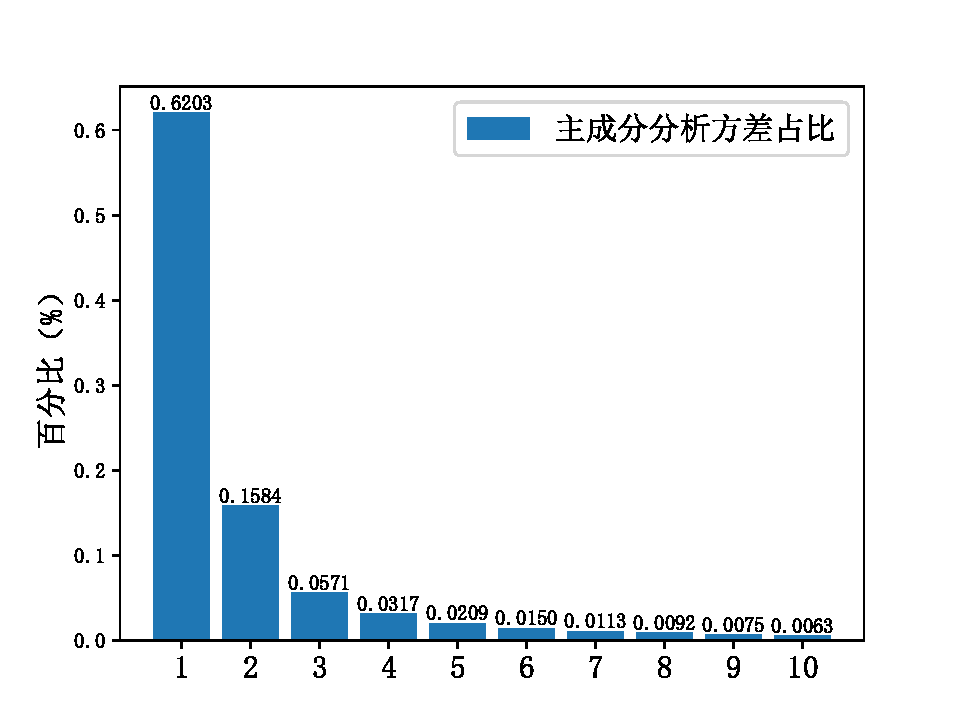
\includegraphics[width=13cm]{histogram.pdf}
    \caption[主成分分析方差占比]
      {在CIFAR-10上训练Resnet-20的前40个轮次训练轨迹在主成分分析(PCA)降维后,前10个主要维度/方向的方差占比。}
   \label{fig:dldr:pca_ratio}
  \end{figure}
  

在训练阶段中,目标子空间中低秩训练的训练集准确度变化如图\ref{fig:dldr:training}所示。从图中可以观察到,低秩降维训练情况下,模型能够相对常规随机梯度下降方法能够更快收敛。

\begin{figure}[!htp]
    \centering
    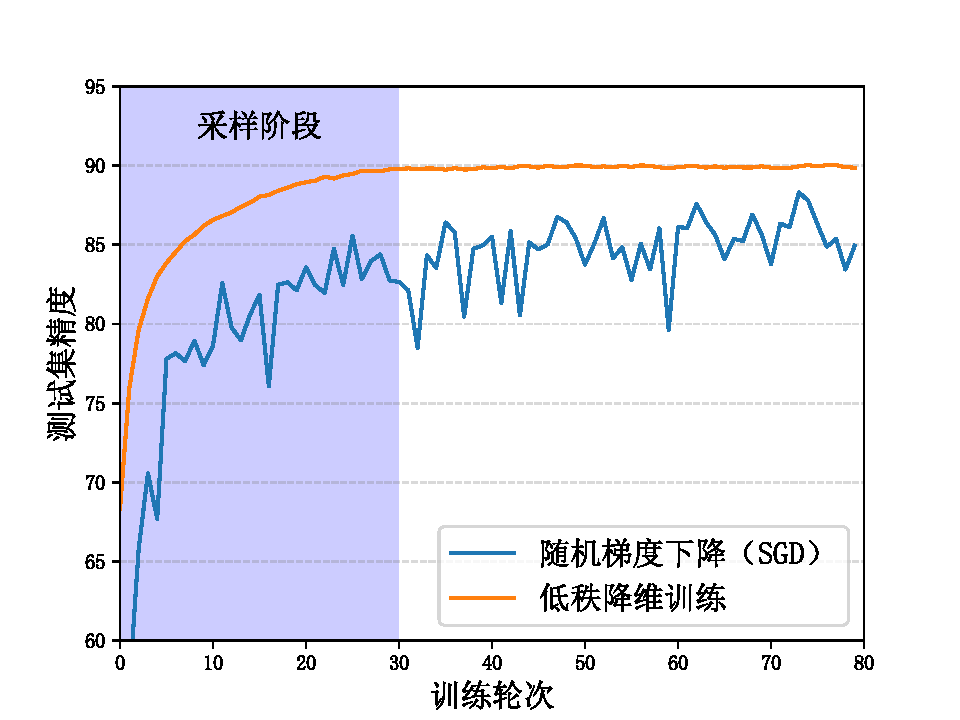
\includegraphics[width=13cm]{sgd_psgd_acc.pdf}
    \caption[中心化低秩降维实验测试集精度变化]
      {随机梯度下降(SGD)和低秩降维训练在CIFAR-10上训练Resnet-20的测试集精度变化}
   \label{fig:dldr:training}
  \end{figure}

在低秩训练的第$7$轮,模型训练集精度已达到并超过采样阶段结束时(第$40$轮)的精度,这表明低秩训练算法能够超越采样阶段结果的限制,从数据中持续学习到更多的信息以提升分类能力。

在低秩训练的第$20$轮,模型训练精度已超过常规随机梯度下降训练结束时的精度,且在后续的训练中继续收敛,最终达到$90.03\%$的精度。这表明低秩训练情况下,模型能达到乃至超过在同等超参数下的随机梯度下降训练的性能。这一性能上的优越性可能来源于低秩降维过程所带来的降噪效果(de-noising),这一点可以在未来进行深入探究。

以上结果表明,我们能够以相当低的维度在CIFAR-10上高效地训练Resnet-20,在一定程度上为低维轨迹假设\ref{hyp:low_dimensional}提供有力支持。

\section{本章小结}

在本章中,我们介绍了给本文后续研究提供主要参考的低维轨迹假设(即假设\ref{hyp:low_dimensional})。为了对该假设进行验证,本章介绍了动态线性降维方法(DLDR,即算法\ref{algo:dldr}),给出基于模型训练轨迹的低秩降维方法。根据该降维方法,本章给出了基于轨迹降维的训练算法,分为采样、降维、训练三个阶段。在验证性实验部分,本文给出了使用Resnet-20结构在CIFAR-10上按照基于轨迹降维的训练算法的实验设计,在实验结果中观察到了该训练算法下能够在低秩子空间进行训练的能力,且性能相比常规随机梯度下降方法在收敛速度、精度上有一定优势。通过本章的研究,我们能在一定的模型、数据集条件下支持低维轨迹假设,且给出一个实现的思路,为后文在联邦学习场景下进行降维压缩打下坚实的基础。



